\documentclass{article}

\usepackage[utf8]{inputenc}
\usepackage[spanish]{babel}
\usepackage{geometry}
\usepackage{graphicx}
\usepackage{titlesec}
\usepackage{lipsum}
\usepackage[dvipsnames]{xcolor}
\usepackage[fleqn]{mathtools}
\usepackage{booktabs}
\usepackage{amsmath}
\usepackage{latexsym}
\usepackage{nccmath}
\usepackage{multicol}
\usepackage{listings}
\usepackage{tasks}
\usepackage{color}
\usepackage{float}
\usepackage{enumitem}
\usepackage{longtable}
\usepackage{makecell}
\usepackage{caption}
\usepackage[parfill]{parskip}
\usepackage{lipsum}
\usepackage{enumitem}
\usepackage{tikz-uml}
\usepackage{hyperref}% Para manejar enlaces


%Definicion de colores
\definecolor{colorIPN}{rgb}{0.5, 0.0,0.13}
\definecolor{colorESCOM}{rgb}{0.0, 0.5,1.0}
\definecolor{myorange}{RGB}{255, 204, 153}
\graphicspath{ {imagenes/} }

% Configuración de la portada
\titleformat{\section}[block]{\normalfont\huge\bfseries}{\thesection}{1em}{}
\geometry{a4paper, margin=1in}

% Definir comandos para información repetitiva
\newcommand{\logoInstitucion}{logotipo_ipn.png} % Reemplaza con el nombre del archivo de tu logo
\newcommand{\logoUniversidad}{EscudoESCOM.png} % Reemplaza con el nombre del archivo de tu logo
\newcommand{\nombreInstituto}{Instituto Politecnico Nacional}
\newcommand{\facultad}{Escuela Superior de Computo}
\newcommand{\materia}{Análisis y Diseño de Sistemas}
\newcommand{\grupo}{4BM1}
\newcommand{\profesora}{Méndez Segundo Laura}
\newcommand{\periodo}{2024/01}
\newcommand{\alumno}{Carrillo Barreiro José Emiliano}

% Definir nuevas listas para información repetitiva
\newlist{bracketed}{enumerate}{1}
\setlist[bracketed,1]{label={[{\arabic*}]},left=0pt}
\begin{document}

% Portada
\begin{titlepage}
    \begin{center}
        \vspace*{1cm}

        \includegraphics[width=0.25\textwidth]{\logoInstitucion}

        \vspace{1cm}

        \textbf{\LARGE \nombreInstituto} \\
        \textbf{\Large \facultad} \\
        \vspace{0.5cm}
        \textbf{\large Materia: \materia} \\
        \textbf{\large Grupo: \grupo} \\
        \vspace{0.5cm}
        \textbf{\large Profesora: \profesora} \\
        \textbf{\large Periodo: \periodo} \\

        \vspace{1cm}

        \textbf{\LARGE Documentacion del Proyecto:} \\
        \vspace{0.5cm}
        \textbf{\Large Plataforma Integral para el Reporte, Análisis y Prevención de Crímenes en la Ciudad de México y Área Metropolitana} \\

        \vfill

        \textbf{\large Realizado por:} \\
        \textbf{\large \alumno \\Huerta Villanueva Oscar  \\Martínez Méndez Diego  \\Reyes Vello Alan Fernando }

        \vspace{1cm}

        \includegraphics[width=0.4\textwidth]{\logoUniversidad}

        \vspace{1cm}

        \textbf{\large \facultad} \\
        \textbf{\large Fecha: \today}

    \end{center}
\end{titlepage}

% Índice
\tableofcontents
\newpage
\listoftables
\listoffigures
\newpage

% Contenido del experimento
\section{Propuesta de Solución}
En la actualidad, nos enfrentamos a una era en la que la toma de decisiones está intrínsecamente ligada a la disponibilidad y eficacia de los datos. Esta necesidad no solo es relevante en el ámbito empresarial o gubernamental, sino que se extiende a diversas esferas, siendo la seguridad ciudadana una de las áreas más críticas. La creciente interconexión global y el aumento exponencial de información en línea plantean el desafío de cómo podemos aprovechar eficientemente la interacción de los usuarios para obtener datos valiosos y representarlos de manera efectiva.
\\
\\En este contexto, el problema que enfrentamos no solo se limita a la recopilación de datos, sino también a la necesidad de convertir esa información en herramientas tangibles que beneficien a la sociedad, específicamente en el ámbito de la seguridad ciudadana. La pregunta clave que surge es: ¿Cómo podemos transformar la participación ciudadana y la información en línea en un recurso efectivo para mejorar la percepción y gestión de la seguridad en nuestras comunidades?
\\
\\La respuesta a este desafío se halla en la creación de un sistema integral que empodere a los ciudadanos en la lucha contra la inseguridad. Este sistema no solo se enfocaría en la recopilación de datos, sino que abarcaría la capacidad de análisis estadístico y la entrega de información procesada de manera accesible. El objetivo es proporcionar a los ciudadanos una herramienta que les permita no solo reportar crímenes, sino también entender las tendencias, visualizar patrones y, lo más crucial, mantenerse informados sobre la seguridad en tiempo real en su entorno inmediato.
\\
\\Al profundizar en el problema, se revela que no se trata solo de crear un mecanismo para la recolección pasiva de datos sobre crímenes, sino de fomentar la participación activa de la comunidad en la construcción de un entorno más seguro. Esto implica la necesidad de establecer un sistema de retroalimentación que involucre a los ciudadanos en el proceso de análisis y mejora continua del sistema, promoviendo así una colaboración efectiva entre la sociedad y las autoridades encargadas de la seguridad.
\\
\\En resumen, el problema va más allá de simplemente obtener información; se trata de empoderar a la comunidad para que participe activamente en la construcción de entornos seguros. La solución no solo yace en la tecnología y la recopilación de datos, sino en la creación de un ecosistema que fomente la transparencia, la colaboración y la toma de decisiones informada para abordar eficazmente los desafíos de la seguridad ciudadana en el mundo moderno.

\section{Propuesta de Solución}
En respuesta al creciente desafío de la seguridad ciudadana en la Ciudad de México, proponemos una solución integral y avanzada que no solo permitirá a los ciudadanos reportar crímenes de manera efectiva, sino que también utilizará tecnología de vanguardia para analizar datos, clasificar incidentes y proporcionar información relevante en tiempo real.

    \subsection{Desarrollo de la Plataforma Web.}
    La plataforma web será una interfaz intuitiva y fácil de usar, diseñada para promover la participación ciudadana y simplificar el proceso de reporte de crímenes. Los usuarios podrán acceder a la plataforma desde sus dispositivos móviles o computadoras, garantizando una amplia accesibilidad. Se implementará un sistema de autenticación seguro para proteger la integridad de los datos y fomentar la confianza de los usuarios en la plataforma.

    \subsection{Sistema de Base de Datos Avanzado.}
    La columna vertebral de nuestra solución será un sistema de base de datos robusto y eficiente. Esta base de datos almacenará de manera segura y organizada todos los informes de crímenes proporcionados por los usuarios, junto con detalles como la fecha, hora, ubicación y descripción del incidente. La base de datos permitirá búsquedas rápidas, análisis históricos y generación de informes para las autoridades pertinentes.

    \subsection{Integración de Software Especializado:}
    Para llevar a cabo el análisis de datos y la clasificación de incidentes, integraremos un software especializado que hará uso de algoritmos avanzados de análisis de patrones y procesamiento de datos. Estos algoritmos permitirán la identificación de tendencias, la categorización precisa de los crímenes y la generación de estadísticas detalladas. Además, se implementarán medidas de aprendizaje automático para mejorar continuamente la precisión del sistema a medida que se recopila más información.

    \subsection{Interactividad a través de Mapa Visual:}
    La plataforma ofrecerá a los usuarios la capacidad de visualizar la distribución de crímenes en la Ciudad de México a través de un mapa interactivo. Este mapa proporcionará una representación visual clara y detallada de las áreas afectadas, permitiendo a los usuarios identificar patrones geoespaciales y a las autoridades enfocar sus esfuerzos de manera estratégica. La interactividad del mapa permitirá filtros por tipo de crimen, intervalos de tiempo y otras variables relevantes.

    \subsection{Sección de Noticias Dinámica:}
    Para mantener a los usuarios informados y concienciados sobre la situación de seguridad en tiempo real, incorporaremos una sección de noticias dinámica. Aquí, se publicarán actualizaciones sobre eventos relevantes, acciones tomadas por las autoridades y consejos de seguridad. Esta sección servirá como un canal de comunicación bidireccional, permitiendo a los usuarios comentar, hacer preguntas y recibir respuestas de las autoridades.

    \subsection{Enfoque en la Participación Ciudadana:}
    La plataforma no solo se centrará en la recopilación de datos, sino que también fomentará la participación ciudadana activa. Se implementarán funciones de retroalimentación para que los usuarios informen sobre la eficacia de las medidas tomadas y sugieran posibles mejoras. Además, se establecerán mecanismos de reconocimiento para destacar la contribución significativa de los ciudadanos a la seguridad comunitaria.

    \subsection{Enlace con Autoridades Competentes:}
    Para garantizar la eficacia de la plataforma, se establecerán conexiones directas con las autoridades competentes, como la policía y las agencias gubernamentales encargadas de la seguridad. La información recopilada estará disponible para estas entidades de manera segura y en tiempo real, permitiendo una respuesta rápida y coordinada ante situaciones críticas.
\\\\
Con esta propuesta, no solo aspiramos a proporcionar una herramienta eficaz para el reporte y análisis de crímenes, sino a fortalecer la colaboración entre la comunidad y las autoridades, contribuyendo así a la construcción de un entorno más seguro y confiable para todos los habitantes de la Ciudad de México.

\section{Objetivo del Sistema}
    \subsection{¿Qué hace el sistema?}

        \subsubsection{Reporte de Crímenes.}
        El sistema permite a los usuarios reportar de manera detallada cualquier incidente delictivo que hayan presenciado o del que tengan conocimiento. La función de reporte incluye la posibilidad de adjuntar información relevante, como descripciones de eventos, fotos o videos, para proporcionar una visión completa y precisa de la situación.

        \subsubsection{Análisis y Visualización.}
        A través de avanzados algoritmos de análisis de datos, el sistema procesa la información recopilada para identificar patrones, tendencias y áreas críticas en términos de actividad criminal. La visualización se realiza de manera interactiva en un mapa, permitiendo a los usuarios comprender la distribución geográfica de los crímenes y tomar decisiones informadas basadas en datos actualizados.

        \subsubsection{Sección de Noticias.}
        La plataforma no solo sirve como un medio para la recopilación de datos, sino también como una fuente de noticias relacionadas con la seguridad en la Ciudad de México. Esta sección se mantiene actualizada con eventos relevantes, medidas gubernamentales y consejos de seguridad, brindando a los usuarios una visión integral del panorama de seguridad en tiempo real.

    \subsection{¿Cómo lo hace?}

        \subsubsection{Interfaz Web.}
        La interfaz web proporciona a los usuarios una experiencia intuitiva y fácil de usar. Permite cargar informes de manera eficiente, acceder a datos actualizados y recibir notificaciones relevantes. La plataforma garantiza la accesibilidad para fomentar la participación activa de los ciudadanos en la construcción de un entorno más seguro.

        \subsubsection{Base de Datos.}
        La información recopilada a través de los informes de crímenes se almacena de manera segura en una base de datos centralizada. Esta base de datos no solo actúa como un repositorio, sino que también permite realizar análisis en profundidad y generar informes estadísticos. La ubicación geográfica de los incidentes se registra meticulosamente para su posterior visualización.

        \subsubsection{Software de Análisis.}
        El sistema implementa un software especializado que utiliza algoritmos avanzados de reconocimiento de patrones y procesamiento de datos. Este software no solo clasifica los informes de crímenes, sino que también identifica correlaciones y tendencias, brindando una comprensión más profunda de la dinámica delictiva en la ciudad.

    \subsection{Público Dirigido.}

        \subsubsection{Ciudadanos preocupados por la seguridad.}
        La plataforma está diseñada para involucrar activamente a los ciudadanos en la vigilancia y mejora de la seguridad en su entorno inmediato.

        \subsubsection{Autoridades gubernamentales encargadas de la aplicación de la ley.}
        Proporciona a las autoridades una herramienta efectiva para acceder a datos actualizados y realizar análisis estratégicos que respalden la toma de decisiones en materia de seguridad.

        \subsubsection{Medios de comunicación interesados en informar sobre la situación de seguridad.}
        La sección de noticias se convierte en una fuente confiable de información para los medios, facilitando la cobertura objetiva y precisa de eventos relacionados con la seguridad en la ciudad.

        \subsubsection{Investigadores y analistas que buscan datos para estudios criminológicos.}
        La plataforma se convierte en una valiosa fuente de datos para aquellos involucrados en la investigación criminológica, proporcionando información detallada sobre patrones delictivos y tendencias a lo largo del tiempo.
        \\\\
        El sistema tiene como objetivo proporcionar una solución integral para la clasificación y organización de imágenes, lo que permite a una amplia gama de usuarios aprovechar eficazmente datos visuales para la toma de decisiones y otros fines específicos.

\section{Objetivos Particulares}
    \subsection{Reporte Ciudadano de Crímenes}
    La plataforma se orienta hacia la facilitación del reporte ciudadano de crímenes, permitiendo a los usuarios ingresar información detallada sobre incidentes delictivos. A través de una interfaz amigable, los ciudadanos podrán contribuir a la construcción de una base de datos robusta para la toma de decisiones informadas en materia de seguridad.

    \subsection{Análisis y Visualización de Datos Criminales.}
    Se implementará un sistema de análisis avanzado que utilizará algoritmos especializados para identificar patrones y tendencias en los datos criminales recopilados. La información se presentará visualmente a través de mapas interactivos, proporcionando una comprensión clara de la distribución geográfica de los crímenes en la ciudad y su área metropolitana.

    \subsection{Prevención y Participación Ciudadana.}
    Además de ser una herramienta para el reporte y análisis, la plataforma fomentará la participación ciudadana en la prevención de crímenes. Se incorporarán funcionalidades que permitan a los usuarios acceder a recursos educativos sobre seguridad, recibir alertas preventivas y colaborar con las autoridades para fortalecer la seguridad comunitaria.

    \subsection{Registro de Incidentes Específicos.}
    El sistema permitirá a los usuarios reportar incidentes específicos, como situaciones de emergencia, puntos de alto riesgo o eventos delictivos recurrentes. Estos registros detallados contribuirán a la generación de informes específicos para la implementación de estrategias de prevención y respuesta más efectivas.

    \subsection{Análisis de Factores Contextuales.}
    Se llevará a cabo un análisis integral que no solo se centrará en los datos criminales, sino también en los factores contextuales que podrían influir en la ocurrencia de crímenes. Esto incluirá variables como iluminación, densidad poblacional y actividades sociales para brindar una perspectiva completa y respaldar la toma de decisiones informada.

    \subsection{Participación Activa de la Comunidad.}
    La plataforma incentivará la participación activa de la comunidad al proporcionar un espacio para la discusión, intercambio de información y colaboración en proyectos comunitarios de seguridad. La creación de una red conectada de ciudadanos contribuirá a fortalecer el tejido social y mejorar la eficacia de las medidas preventivas.

\section{Metodología.}
En la creación de la plataforma integral para el reporte, análisis y prevención de crímenes en la Ciudad de México y Área Metropolitana, es fundamental seguir una metodología estructurada que garantice la eficacia y la satisfacción de los usuarios. El desarrollo se llevará a cabo a través de la siguiente metodología:

    \subsection{Investigación y Análisis.}
       \begin{itemize}
           \item Recopilación de información sobre las necesidades específicas de los usuarios y las características del entorno urbano.
           \item Análisis de plataformas existentes para identificar mejores prácticas y posibles mejoras.
       \end{itemize}

    \subsection{Desarrollo de la Plataforma.}
        \begin{itemize}
            \item Implementación de un sistema de reporte intuitivo y fácil de usar.
            \item Integración de algoritmos avanzados para el análisis y clasificación de datos relacionados con crímenes.
            \item Desarrollo de una interfaz interactiva para el usuario, incluyendo un mapa geográfico para visualizar los datos.
        \end{itemize}

    \subsection{Prevención y Toma de Decisiones.}
        \begin{itemize}
            \item Incorporación de herramientas predictivas para la prevención de crímenes basadas en análisis de patrones históricos.
            \item Creación de paneles de control personalizados para facilitar la toma de decisiones basada en los datos recopilados.
        \end{itemize}

    \subsection{Cuestionario para el Usuario.}
        \begin{enumerate}[label=\arabic*.]
            \item \textbf{¿Con qué frecuencia experimenta situaciones de seguridad o crímenes en su área de residencia o trabajo?}
                \begin{enumerate}[label=\alph*)]
                \item Diariamente.
                \item Semanalmente.
                \item Mensualmente.
                \item Raramente.
                \item Nunca.
                \end{enumerate}
            \item \textbf{¿Cómo se siente actualmente acerca de la eficacia de los métodos de reporte de crímenes disponibles en su ciudad?}
                \begin{enumerate}[label=\alph*.]
                    \item Muy efectivos.
                    \item Efectivos.
                    \item Neutrales.
                    \item Inefectivos.
                    \item Muy inefectivos.
                \end{enumerate}

            \item \textbf{¿Qué tipo de información considera más relevante al reportar un crimen o incidente de seguridad?}
                \begin{enumerate}[label=\alph*.]
                    \item Ubicación.
                    \item Hora.
                    \item Descripción.
                    \item Involucrados.
                    \item Otro (por favor, especificar).
                \end{enumerate}

            \item \textbf{¿Cuál es su nivel de confianza en las fuerzas de seguridad y en la capacidad del gobierno para abordar y prevenir delitos en su área?}
                \begin{enumerate}[label=\alph*.]
                    \item Muy confiado.
                    \item Confiado.
                    \item Neutro.
                    \item Poco confiado.
                    \item Nada confiado.
                \end{enumerate}

            \item \textbf{¿En qué medida utiliza actualmente tecnologías o aplicaciones para mantenerse informado sobre la seguridad en su entorno?}
                \begin{enumerate}[label=\alph*.]
                    \item Frecuentemente.
                    \item Ocasionalmente.
                    \item Raramente.
                    \item Nunca.
                    \item No estoy seguro.
                \end{enumerate}

            \item \textbf{¿Qué características o funcionalidades le gustaría ver en una plataforma integral para el reporte y análisis de crímenes?}
                \begin{enumerate}[label=\alph*.]
                    \item Interfaz fácil de usar.
                    \item Mapas interactivos.
                    \item Estadísticas de crímenes en tiempo real.
                    \item Reportes anónimos.
                    \item Otro (por favor, especificar).
                \end{enumerate}

            \item \textbf{¿Qué barreras o preocupaciones tendría al utilizar una plataforma en línea para reportar crímenes?}
                \begin{enumerate}[label=\alph*.]
                    \item Falta de privacidad.
                    \item Temor a represalias.
                    \item Desconfianza en la seguridad de la plataforma.
                    \item Complejidad en el proceso de reporte.
                    \item Ninguna preocupación.
                \end{enumerate}

            \item \textbf{¿Consideraría importante la inclusión de funciones de análisis de datos para identificar patrones de criminalidad en su área?}
                \begin{enumerate}[label=\alph*.]
                    \item Muy importante.
                    \item Importante.
                    \item Neutro.
                    \item Poco importante.
                    \item Nada importante.
                \end{enumerate}

            \item \textbf{¿Cómo cree que la participación ciudadana puede mejorar la seguridad en su comunidad?}
                \begin{enumerate}[label=\alph*.]
                    \item Vigilancia comunitaria.
                    \item Colaboración con las autoridades.
                    \item Participación en programas de prevención.
                    \item Información y concientización.
                    \item Otro (por favor, especificar).
                \end{enumerate}

            \item \textbf{¿Estaría dispuesto(a) a colaborar activamente en la prevención de crímenes a través de una plataforma, por ejemplo, compartiendo información o participando en iniciativas comunitarias?}
                \begin{enumerate}[label=\alph*.]
                    \item Sí, definitivamente.
                    \item Sí, posiblemente.
                    \item No estoy seguro(a).
                    \item No, probablemente no.
                    \item No, definitivamente no.
                \end{enumerate}

        \end{enumerate}
Este cuestionario nos permitirá personalizar la plataforma según las necesidades y expectativas de los usuarios, asegurando un producto integral y efectivo.

\section{Requerimientos.}
\begin{table}
  \centering
  \caption{Tabla de Requerimientos}
  \label{Requerimientos}
  \resizebox{\textwidth}{!}{%
      \begin{tabular}{|c|c|c|c|c|c|}
        \hline
         \textbf{Núm.} & \textbf{Caso de Uso.} & \textbf{Actores.} & \textbf{Condicion Inicial.} & \textbf{Secuencia Eventos.} & \textbf{Evento final.} \\
        \hline
        01 &
            \begin{tabular}{@{}c@{}}
             Registrar \\
             Usuario.
            \end{tabular}& Cliente. &
            \begin{tabular}{@{}c@{}}
             El Cliente no tiene \\
             cuenta en la plataforma.
            \end{tabular} &
            \begin{tabular}{@{}c@{}}
             Registar Datos. \\
             Almacenar Datos.
            \end{tabular}&
            \begin{tabular}{@{}c@{}}
             Se crea \\
             nuevo cliente
            \end{tabular} \\
        \hline
        02 &
            \begin{tabular}{@{}c@{}}
             Iniciar \\
             Sesion.
            \end{tabular}&
            \begin{tabular}{@{}c@{}}
             Cliente \\
             Admin.
            \end{tabular}&
            \begin{tabular}{@{}c@{}}
             El Usuario entra \\
             a la pagina.
            \end{tabular}&
            \begin{tabular}{@{}c@{}}
             Ingresa Datos. \\
             Se verifican Datos.
            \end{tabular}&
            \begin{tabular}{@{}c@{}}
             El Usuario entra \\
             a la pagina.
            \end{tabular}\\
        \hline
        03 &
            \begin{tabular}{@{}c@{}}
             Levantar \\
             Reporte.
            \end{tabular}& Cliente. &
            \begin{tabular}{@{}c@{}}
             El Cliente desea \\
             levantar reporte \\
             estando en la pagina.
            \end{tabular} &
            \begin{tabular}{@{}c@{}}
             Ir a Reporta.\\
             Registar Datos.\\
             Almacenar Datos.
            \end{tabular}&
            \begin{tabular}{@{}c@{}}
             Se crea \\
             nuevo reporte
            \end{tabular} \\
        \hline
        04 &
            \begin{tabular}{@{}c@{}}
             Checar \\
             Mapa.
            \end{tabular}& Cliente. &
            \begin{tabular}{@{}c@{}}
             El Cliente desea \\
             Checar Mapa \\
             estando en la pagina.
            \end{tabular} &
            \begin{tabular}{@{}c@{}}
             Dirigirse a \\
             opcion "Mapa".
            \end{tabular}&
            \begin{tabular}{@{}c@{}}
             Se visualiza \\
             el mapa.
            \end{tabular}\\
        \hline
        05 &
            \begin{tabular}{@{}c@{}}
             Checar \\
             Noticias.
            \end{tabular}& Cliente. &
        \begin{tabular}{@{}c@{}}
             El Cliente desea \\
             Checar Noticias \\
             estando en la pagina.
            \end{tabular} &
            \begin{tabular}{@{}c@{}}
             Dirigirse a \\
             opcion "Noticias".
            \end{tabular}&
            \begin{tabular}{@{}c@{}}
             se visualizan \\
             las noticias.
            \end{tabular}\\
        \hline
        06 &
            \begin{tabular}{@{}c@{}}
             Revisar \\
             Reportes.
            \end{tabular}. & Cliente. &
            \begin{tabular}{@{}c@{}}
             El Cliente desea \\
             Revisar Reporte \\
             estando en la pagina.
            \end{tabular} &
            \begin{tabular}{@{}c@{}}
             Dirigirse a \\
             opcion "Recientes".
            \end{tabular}&
            \begin{tabular}{@{}c@{}}
             Se visualizan \\
             reportes\\recientes.
            \end{tabular}\\
        \hline
        07 &
            \begin{tabular}{@{}c@{}}
             Visualizar \\
             Reporte.
            \end{tabular}& Cliente. &
            \begin{tabular}{@{}c@{}}
             El Cliente desea \\
             visualizar sus reportes \\
             estando en la pagina.
            \end{tabular}&
            \begin{tabular}{@{}c@{}}
             -Ir a "Perfil". \\
             -Ir a "Crimenes\\Reportados".\\
             -Dar click al reporte.
            \end{tabular}&
            \begin{tabular}{@{}c@{}}
             Se vizualiza \\
             reporte.
            \end{tabular}\\
        \hline
        08 &
            \begin{tabular}{@{}c@{}}
             Actualizar \\
             Reporte.
            \end{tabular}& Cliente. &
            \begin{tabular}{@{}c@{}}
             El Cliente desea \\
             actualizar reporte \\
             estando en la pagina.
            \end{tabular}&
            \begin{tabular}{@{}c@{}}
             -Ir a "Perfil". \\
             -Ir a "Crimenes\\Reportados".\\
             -Dar click al reporte\\a actualizar.\\
             -Rellenar Datos.\\
             -Almacenar Datos.
            \end{tabular}&
            \begin{tabular}{@{}c@{}}
             Se actualiza \\
             reporte.
            \end{tabular}\\
        \hline
        09 &
            \begin{tabular}{@{}c@{}}
             Eliminar \\
             Reporte.
            \end{tabular}& Cliente. &
            \begin{tabular}{@{}c@{}}
             El Cliente desea \\
             eliminar reporte \\
             estando en la pagina.
            \end{tabular} &
            \begin{tabular}{@{}c@{}}
             -Ir a "Perfil". \\
             -Ir a "Crimenes\\Reportados".\\
             -Dar click al  ID del\\reportea eliminar.\\
             -Inhabilitar acceso\\a Datos.
            \end{tabular}&
            \begin{tabular}{@{}c@{}}
             Se "elimina" \\
             reporte.
            \end{tabular}\\
        \hline
        10 &
            \begin{tabular}{@{}c@{}}
             Checar \\
             Localidad.
            \end{tabular}& Cliente. &
            \begin{tabular}{@{}c@{}}
             El Cliente desea \\
             Checar lugar del\\
             reprote estando\\
             en la pagina.
            \end{tabular}&
            \begin{tabular}{@{}c@{}}
             -Ir a "Perfil/\\Crimenes Reportados"\\ o ir a "Recientes".\\
             -Dar click al  ID del\\reporte a checar\\
            \end{tabular}&
            \begin{tabular}{@{}c@{}}
             Se visualiza \\
             lugar del\\reporte.
            \end{tabular}\\
        \hline
        11 &
        \begin{tabular}{@{}c@{}}
             Actualizar \\
             Img Usuario.
            \end{tabular}&
        \begin{tabular}{@{}c@{}}
             Cliente \\
             Admin.
            \end{tabular} &
            \begin{tabular}{@{}c@{}}
             El Usuario desea \\
             actualizar su imagen \\
             estando en la pagina.
            \end{tabular}&
            \begin{tabular}{@{}c@{}}
             -Ir a "Perfil". \\
             -Ir a "Imagen\\de perfil".\\
             -Subir imagen.\\
             -Almacenar Imagen
            \end{tabular}&
            \begin{tabular}{@{}c@{}}
             Se actualiza \\
             imagen de Us.
            \end{tabular}\\
        \hline
        12 &
        \begin{tabular}{@{}c@{}}
             Verificar \\
             Reporte.
            \end{tabular}& Admin. &
            \begin{tabular}{@{}c@{}}
             Admin debe \\
             Verificar reporte \\
             estando en la pagina.
            \end{tabular}&
            \begin{tabular}{@{}c@{}}
             -Dirigirse a \\
             opcion "Recientes".\\
             -Comprobar Info.
            \end{tabular}&
            \begin{tabular}{@{}c@{}}
             Aprobar \\
             Reporte.
            \end{tabular}\\
        \hline
        13 &
        \begin{tabular}{@{}c@{}}
             Dar de baja \\
             reporte.
            \end{tabular}& Admin. &
            \begin{tabular}{@{}c@{}}
             Admin debe \\
             dar de baja reporte \\
             estando en la pagina.
            \end{tabular}&\begin{tabular}{@{}c@{}}
             -Dirigirse a \\
             opcion "Antiguos".\\
             -Comprobar antiguedad.
            \end{tabular}&
            \begin{tabular}{@{}c@{}}
             Borrar \\
             datos.
            \end{tabular}\\
        \hline
      \end{tabular}
    }
\end{table}

La Tabla de Requerimientos\ref{Requerimientos} muestra el desglose de los casos de uso que tiene el sistema..


\section{Calendarización.}
    \begin{figure}[H]
        \centering
        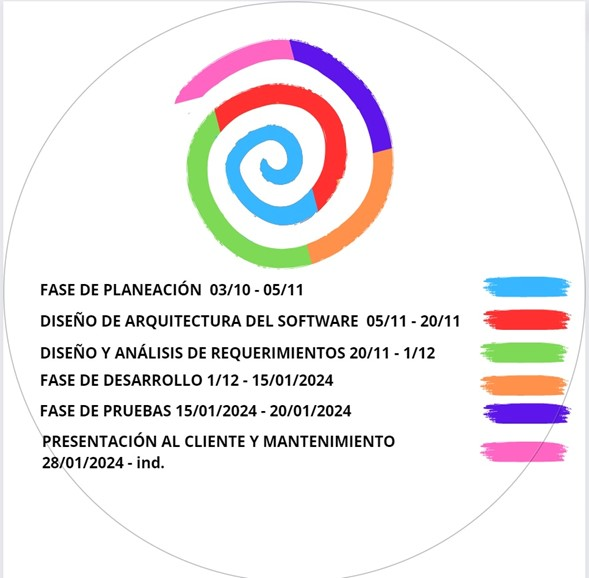
\includegraphics[width=1\linewidth]{Sin título.jpg}
        \caption{Calendario de Entregas del Sistema. Modelo Espiral}
        \label{fig:enter-label}
    \end{figure}
\section{Diagramas.}
    \subsection{Diagrama de Clases.}
    \subsection{Diagrama de Casos de Uso.}
    \begin{figure} [H]
                \begin{center}
                    \begin{tikzpicture}[scale = 0.7]
                      \begin{umlsystem}{Sistema}
                        \umlusecase[name=caso1, x=6, y=0]{\small Registrar Usuario}
                        \umlusecase[name=caso2,x=6,y=-2]{\small Iniciar Sesión}
                        \umlusecase[name=caso3, y=0]{\small Levantar Reporte}
                        \umlusecase[name=caso4, y = -2]{\small Checar Mapa}
                        \umlusecase[name=caso5,y=-4]{\small Checar Noticias}
                        \umlusecase[name=caso6, y= -6]{\small Revisar Reporte}
                        \umlusecase[name=caso7,x=6,y=-9]{\small Actualizar Reporte}
                        \umlusecase[name=caso8,x=3,y=-11]{\small Eliminar Reporte}
                        \umlusecase[name=caso9,x=8,y=-7]{\small Checar Localidad}
                        \umlusecase[name=caso10,y=-8]{\small Visualizar Reporte}
                        \umlusecase[name=caso11,x=6,y=-5]{\small Actualizar Img Usuario}
                        \umlusecase[name=caso12,x=12,y=-9]{\small Verificar Reporte}
                        \umlusecase[name=caso13,x=12]{\small Dar de Baja Reporte}

                        % Inclusion
                        \umlinclude{caso10}{caso7}
                        \umlinclude{caso10}{caso8}
                        \umlinclude{caso10}{caso9}
                        \umlinclude{caso6}{caso9}

                        % Extension
                        \umlVHVextend{caso1}{caso2}
                      \end{umlsystem}

                      % Actores
                      \umlactor[x=-5 , y=-5]{Cliente}
                      \umlactor[x=17 , y=-5]{Admin}

                      % Asociaciones entre actores y casos de uso
                      \umlassoc{Cliente}{caso2}
                      \umlassoc{Cliente}{caso3}
                      \umlassoc{Cliente}{caso4}
                      \umlassoc{Cliente}{caso5}
                      \umlassoc{Cliente}{caso6}
                      \umlassoc{Cliente}{caso10}
                      \umlassoc{Cliente}{caso11}

                      \umlassoc{Admin}{caso2}
                      \umlassoc{Admin}{caso11}
                      \umlassoc{Admin}{caso12}
                      \umlassoc{Admin}{caso13}
                    \end{tikzpicture}
                \caption{Diagrama de Casos de Uso del Sistema.}
                \end{center}
            \end{figure}
    \subsection{Diagramas de Secuencia.}
        \subsubsection{Registrar Usuario.}
            \begin{figure} [H]
                \begin{center}
                    \begin{tikzpicture} [scale = 0.9]
                        \begin{umlseqdiag}
                        \umlactor[class=Persona]{Actor}
                        \umlboundary[class = Computadora]{Frontera}
                        \umlcontrol[class=Ctrl]{Controlador}
                        \umldatabase[class=Base de Datos]{DB}
                        \umlentity[class=Usuario]{Entidad}

                        \begin{umlcall}[dt=5,op=Abrir(Pagina), type=synchron, return= Mostrar(Pagina)]{Actor}{Frontera}
                        \begin{umlcall}[dt=5,op=Acceder(servidor), type=synchron, return= Archivos]{Frontera}{Controlador}
                        \end{umlcall}
                        \end{umlcall}
                        \begin{umlcall}[dt=5 , op=Seleccionar(Registrarse), type synchron, return= Pagina(Registro)]{Actor}{Frontera}
                        \begin{umlcall}[dt=5,op=Acceder(servidor), type=synchron, return= Archivos]{Frontera}{Controlador}
                        \end{umlcall}
                        \end{umlcall}
                        \begin{umlcall}[dt=5 , op=Ingresar(Datos), type synchron, return= Mensaje(Exito)]{Actor}{Frontera}
                        \begin{umlcall}[dt=5,op=Mandar(datos), type=synchron, with return]{Frontera}{Controlador}
                        \begin{umlcall}[dt=5,op=Procesar(datos), type=synchron]{Controlador}{Controlador}
                        \begin{umlcall}[dt=5,op=Almacenar(datos), type=synchron, with return]{Controlador}{DB}
                        \begin{umlcall}[dt=5,op=Crear(Usuario), type=synchron, return= Usuario]{DB}{Entidad}
                        \end{umlcall}
                        \end{umlcall}
                        \end{umlcall}
                        \end{umlcall}
                        \end{umlcall}
                        \end{umlseqdiag}
                    \end{tikzpicture}
                \caption{Diagrama de Secuencia Registrar usuario.}
                \end{center}
            \end{figure}
        \subsubsection{Iniciar sesion.}
            \begin{figure} [H]
                \begin{center}
                    \begin{tikzpicture} [scale = 0.9]
                        \begin{umlseqdiag}
                        \umlactor[class=Persona]{Actor}
                        \umlboundary[class = Computadora]{Frontera}
                        \umlcontrol[class=Ctrl]{Controlador}
                        \umldatabase[class=Base de Datos]{DB}
                        \umlentity[class=Usuario]{Entidad}

                        \begin{umlcall}[dt=5,op=Abrir(Pagina), type=synchron, return= Mostrar(Pagina)]{Actor}{Frontera}
                        \begin{umlcall}[dt=5,op=Acceder(servidor), type=synchron, return= Archivos]{Frontera}{Controlador}
                        \end{umlcall}
                        \end{umlcall}
                        \begin{umlcall}[dt=5 , op=Seleccionar(Iniciar Sesión), type synchron, return= Pagina(Iniciar Sesión)]{Actor}{Frontera}
                        \begin{umlcall}[dt=5,op=Acceder(servidor), type=synchron, return= Archivos]{Frontera}{Controlador}
                        \end{umlcall}
                        \end{umlcall}
                        \begin{umlcall}[dt=5 , op=Ingresar(Datos), type synchron]{Actor}{Frontera}
                            \begin{umlcall}[dt=5,op=Mandar(datos), type=synchron]{Frontera}{Controlador}
                                \begin{umlcall}[dt=5,op=Procesar(datos), type=synchron]{Controlador}{Controlador}
                                    \begin{umlcall}[dt=5,op=Consultar(datos), type=synchron]{Controlador}{DB}
                                        \begin{umlcall}[dt=5,op=Buscar(Usuario), type=synchron, padding = 3]{DB}{Entidad}
                                            \begin{umlfragment}[type=alt , label=Invalido , inner xsep=5, padding 5]
                                                \begin{umlcall}[dt=1,op=Not Found, type=synchron]{Entidad}{DB}
                                                \end{umlcall}
                                                \begin{umlcall}[dt=1 type=asynchron]{DB}{Controlador}
                                                \end{umlcall}
                                                \begin{umlcall}[dt=1, type=asynchron, return= Usuario]{Controlador}{Frontera}
                                                \end{umlcall}
                                                \begin{umlcall}[dt=1, op=Pagina(Iniciar Sesión),type=asynchron]{Frontera}{Actor}
                                                \end{umlcall}
                                            \umlfpart[Valido]{}
                                                \begin{umlcall}[dt=15,op=Usuario, type=synchron]{Entidad}{DB}
                                                \end{umlcall}
                                                \begin{umlcall}[dt=5, type=asynchron, return= Usuario]{DB}{Controlador}
                                                \end{umlcall}
                                                \begin{umlcall}[dt=5, type=asynchron, return= Usuario]{Controlador}{Frontera}
                                                \end{umlcall}
                                                \begin{umlcall}[dt=5, op=Pagina(Inicio),type=asynchron]{Frontera}{Actor}
                                                \end{umlcall}
                                            \end{umlfragment}
                                        \end{umlcall}
                                    \end{umlcall}
                                \end{umlcall}
                            \end{umlcall}
                        \end{umlcall}
                        \end{umlseqdiag}
                    \end{tikzpicture}
                \caption{Diagrama de Secuencia Iniciar Sesión.}
                \end{center}
            \end{figure}
        \subsubsection{Levantar reporte.}
            \begin{figure} [H]
                \begin{center}
                    \begin{tikzpicture} [scale = 0.9]
                        \begin{umlseqdiag}
                        \umlactor[class=Persona]{Actor}
                        \umlboundary[class = Computadora]{Frontera}
                        \umlcontrol[class=Ctrl]{Controlador}
                        \umldatabase[class=Base de Datos]{DB}
                        \umlentity[class=Reportar]{Entidad}

                        \begin{umlcall}[dt=5 , op=Seleccionar(Reportar), type synchron, return= Pagina(Reportar)]{Actor}{Frontera}
                        \begin{umlcall}[dt=5,op=Acceder(servidor), type=synchron, return= Formulario]{Frontera}{Controlador}
                        \end{umlcall}
                        \end{umlcall}
                        \begin{umlcall}[dt=5 , op=Ingresar(Datos), type synchron, return= Mensaje(Exito)]{Actor}{Frontera}
                        \begin{umlcall}[dt=5,op=Mandar(datos), type=synchron, with return]{Frontera}{Controlador}
                        \begin{umlcall}[dt=5,op=Procesar(datos), type=synchron]{Controlador}{Controlador}
                        \begin{umlcall}[dt=5,op=Almacenar(datos), type=synchron, with return]{Controlador}{DB}
                        \begin{umlcall}[dt=5,op=Crear(Reporte), type=synchron, return= Exito]{DB}{Entidad}
                        \end{umlcall}
                        \end{umlcall}
                        \end{umlcall}
                        \end{umlcall}
                        \end{umlcall}
                        \end{umlseqdiag}
                    \end{tikzpicture}
                \caption{Diagrama de Secuencia Registrar Reporte.}
                \end{center}
            \end{figure}
        \subsubsection{Checar Mapa.}
        \begin{figure} [H]
                \begin{center}
                    \begin{tikzpicture} [scale = 1.5]
                        \begin{umlseqdiag}
                        \umlactor[class=Persona]{Actor}
                        \umlboundary[class = Computadora]{Frontera}
                        \umlcontrol[class=Ctrl]{Controlador}
                        \begin{umlcall}[dt=5 , op=Seleccionar(Mapa), type synchron, return= Pagina(Mapa)]{Actor}{Frontera}
                            \begin{umlcall}[dt=5,op=Acceder(servidor), type=synchron, return= Mapa]{Frontera}{Controlador}
                            \end{umlcall}
                        \end{umlcall}
                        \end{umlseqdiag}
                    \end{tikzpicture}
                \caption{Diagrama de Secuencia Checar Mapa.}
                \end{center}
        \end{figure}
        \subsubsection{Checar noticias.}
        \begin{figure} [H]
                \begin{center}
                    \begin{tikzpicture} [scale = 1.2]
                        \begin{umlseqdiag}
                        \umlactor[class=Persona]{Actor}
                        \umlboundary[class = Computadora]{Frontera}
                        \umlcontrol[class=Ctrl]{Controlador}
                        \begin{umlcall}[dt=5 , op=Seleccionar(Logo), type synchron, return= Pagina(Principal)]{Actor}{Frontera}
                            \begin{umlcall}[dt=5,op=Acceder(servidor), type=synchron, return= Lista(Noticias)]{Frontera}{Controlador}
                            \end{umlcall}
                        \end{umlcall}
                        \end{umlseqdiag}
                    \end{tikzpicture}
                \caption{Diagrama de Secuencia Checar Noticias.}
                \end{center}
        \end{figure}
        \subsubsection{Revisar reportes.}
        \begin{figure} [H]
                \begin{center}
                    \begin{tikzpicture} [scale = 1.2]
                        \begin{umlseqdiag}
                        \umlactor[class=Persona]{Actor}
                        \umlboundary[class = Computadora]{Frontera}
                        \umlcontrol[class=Ctrl]{Controlador}
                        \begin{umlcall}[dt=5 , op=Seleccionar(Recientes), type synchron, return= Pagina(Recientes)]{Actor}{Frontera}
                            \begin{umlcall}[dt=5,op=Acceder(servidor), type=synchron, return= Lista(Reportes)]{Frontera}{Controlador}
                            \end{umlcall}
                        \end{umlcall}
                        \end{umlseqdiag}
                    \end{tikzpicture}
                \caption{Diagrama de Secuencia Revisar Repores.}
                \end{center}
        \end{figure}
        \subsubsection{Visualizar reporte}
        \begin{figure} [H]
                \begin{center}
                    \begin{tikzpicture} [scale = 1.2]
                        \begin{umlseqdiag}
                            \umlactor[class=Persona]{Actor}
                            \umlboundary[class = Computadora]{Frontera}
                            \umlcontrol[class=Ctrl]{Controlador}
                            \umldatabase[class=Base de Datos]{DB}

                            \begin{umlcall}[dt=5 , op=Seleccionar(ImgUsuario), type synchron, return= Pagina(Crimenes Reportados)]{Actor}{Frontera}
                                \begin{umlcall}[dt=5,op=Acceder(servidor), type=synchron, return= Lista(Reportes)]{Frontera}{Controlador}
                                \end{umlcall}
                            \end{umlcall}
                            \begin{umlcall}[dt=5 , op=Seleccionar(Reporte), type synchron, return= Pagina(Reporte)]{Actor}{Frontera}
                                \begin{umlcall}[dt=5,op=Acceder(servidor), type=synchron, return= Datos(Reporte)]{Frontera}{Controlador}
                                    \begin{umlcall}[dt=5,op=Buscar(Reporte), type=synchron, return= Reporte]{Controlador}{DB}
                                    \end{umlcall}
                                \end{umlcall}
                            \end{umlcall}
                        \end{umlseqdiag}
                    \end{tikzpicture}
                \caption{Diagrama de Secuencia Visualizar Reporte.}
                \end{center}
            \end{figure}
        \subsubsection{Actualizar reportes.}
        \begin{figure} [H]
                \begin{center}
                    \begin{tikzpicture} [scale = 0.75]
                        \begin{umlseqdiag}
                            \umlactor[class=Persona]{Actor}
                            \umlboundary[class = Computadora]{Frontera}
                            \umlcontrol[class=Ctrl]{Controlador}
                            \umldatabase[class=Base de Datos]{DB}
                            \umlentity[class=Reporte]{Entidad}

                            \begin{umlcall}[dt=5 , op=Seleccionar(Actualizar), type synchron, return= Formulario]{Actor}{Frontera}
                                \begin{umlcall}[dt=5,op=Acceder(servidor), type=synchron, return= Lista(Reportes), padding=3]{Frontera}{Controlador}
                                \end{umlcall}
                            \end{umlcall}
                            \begin{umlcall}[dt=5 , op=ingresar(Datos), type synchron, return= Pagina(Reporte)]{Actor}{Frontera}
                                \begin{umlcall}[dt=5,op=Mandar(datos), type=synchron, return= Datos(Reporte)]{Frontera}{Controlador}
                                    \begin{umlcall}[dt=5,op=Procesar(datos), type=synchron]{Controlador}{Controlador}
                                        \begin{umlcall}[dt=5,op=Almacenar(datos), type=synchron, return= Reporte]{Controlador}{DB}
                                            \begin{umlcall}[dt=5,op=Actualizar(Reporte), type=synchron, return= Reporte]{DB}{Entidad}
                                            \end{umlcall}
                                        \end{umlcall}
                                    \end{umlcall}
                                \end{umlcall}
                            \end{umlcall}
                        \end{umlseqdiag}
                    \end{tikzpicture}
                \caption{Diagrama de Secuencia Actualizar Reporte.}
                \end{center}
            \end{figure}
        \subsubsection{Eliminar Reporte.}
        \begin{figure} [H]
                \begin{center}
                    \begin{tikzpicture} [scale = 0.8]
                        \begin{umlseqdiag}
                            \umlactor[class=Persona]{Actor}
                            \umlboundary[class = Computadora]{Frontera}
                            \umlcontrol[class=Ctrl]{Controlador}
                            \umldatabase[class=Base de Datos]{DB}
                            \umlentity[class=Reporte]{Entidad}

                            \begin{umlcall}[dt=7 , op=Seleccionar(Eliminar), type synchron, return= Confirmación]{Actor}{Frontera}
                                \begin{umlcall}[dt=7,op=Acceder(servidor), type=synchron, return= Pagina(Confirmación), padding =3]{Frontera}{Controlador}
                                \end{umlcall}
                            \end{umlcall}
                            \begin{umlfragment}[type=alt , label=Denegar, inner xsep=7, ysep=10]
                                \begin{umlcall}[dt=7 , op=Seleccionar(Denegar), type synchron, return= Pagina(Reporte), padding = 3]{Actor}{Frontera}
                                \end{umlcall}
                            \umlfpart[Aceptar]{}
                                \begin{umlcall}[dt=5 , op=Seleccionar(aceptar), type synchron, return= Pagina(Exito)]{Actor}{Frontera}
                                    \begin{umlcall}[dt=5,op=Mandar(solicitud), type=synchron, with return]{Frontera}{Controlador}
                                        \begin{umlcall}[dt=5,op=Procesar(solicitud), type=synchron]{Controlador}{Controlador}
                                            \begin{umlcall}[dt=5,op=Inhabilitar(datos), type=synchron, return= null]{Controlador}{DB}
                                                \begin{umlcall}[dt=5,op=Inhabilitar(Reporte), type=synchron, return= null]{DB}{Entidad}
                                                \end{umlcall}
                                            \end{umlcall}
                                        \end{umlcall}
                                    \end{umlcall}
                                \end{umlcall}
                            \end{umlfragment}
                        \end{umlseqdiag}
                    \end{tikzpicture}
                \caption{Diagrama de Secuencia Eliminar Reporte.}
                \end{center}
            \end{figure}
        \subsubsection{Checar Localidad}
            \begin{figure} [H]
                \begin{center}
                    \begin{tikzpicture} [scale = 1.2]
                        \begin{umlseqdiag}
                        \umlactor[class=Persona]{Actor}
                        \umlboundary[class = Computadora]{Frontera}
                        \umlcontrol[class=Ctrl]{Controlador}
                        \begin{umlcall}[dt=5 , op=Seleccionar(ID), type synchron, return= Pagina(Mapa)]{Actor}{Frontera}
                            \begin{umlcall}[dt=5,op=Acceder(servidor), type=synchron, return= Lista(Reportes)]{Frontera}{Controlador}
                            \end{umlcall}
                        \end{umlcall}
                        \end{umlseqdiag}
                    \end{tikzpicture}
                \caption{Diagrama de Secuencia Checar Localidad.}
                \end{center}
            \end{figure}
        \subsubsection{Actualizar Img Usuario}
        \begin{figure} [H]
                \begin{center}
                    \begin{tikzpicture} [scale = 0.9]
                        \begin{umlseqdiag}
                            \umlactor[class=Persona]{Actor}
                            \umlboundary[class = Computadora]{Frontera}
                            \umlcontrol[class=Ctrl]{Controlador}
                            \umldatabase[class=Base de Datos]{DB}
                            \umlentity[class =Usuario]{Entidad}

                            \begin{umlcall}[dt=5 , op=Seleccionar(ImgUsuario), type synchron, return= Pagina(Crimenes Reportados)]{Actor}{Frontera}
                                \begin{umlcall}[dt=5,op=Acceder(servidor), type=synchron, return= Lista(Reportes), padding=3]{Frontera}{Controlador}
                                \end{umlcall}
                            \end{umlcall}
                            \begin{umlcall}[dt=5 , op=Seleccionar(CargarImagen), type synchron, return= Pagina(Formulario)]{Actor}{Frontera}
                                \begin{umlcall}[dt=5,op=Acceder(servidor), type=synchron, return = Formulario]{Frontera}{Controlador}
                                \end{umlcall}
                            \end{umlcall}
                            \begin{umlcall}[dt=5,op=Cargar(Imagen), type=synchron, return= Pagina(Exito)]{Actor}{Frontera}
                                \begin{umlcall}[dt=5,op=Mandar(Imagen), type=synchron, return= Exito]{Frontera}{Controlador}
                                    \begin{umlcall}[dt=5,op=Procesar(Imagen), type=synchron]{Controlador}{Controlador}
                                        \begin{umlcall}[dt=5,op=Almacenar(Imagen), type=synchron, return= Exito]{Controlador}{DB}
                                            \begin{umlcall}[dt=5,op=Actualizar(imagen), type=synchron, return= Usuario]{DB}{Entidad}
                                            \end{umlcall}
                                        \end{umlcall}
                                    \end{umlcall}
                                \end{umlcall}
                            \end{umlcall}
                        \end{umlseqdiag}
                    \end{tikzpicture}
                \caption{Diagrama de Secuencia Actualizar Imagen de Usuario.}
                \end{center}
            \end{figure}
        \subsubsection{Verificar Reporte}
            \begin{figure} [H]
                \begin{center}
                    \begin{tikzpicture} [scale = 0.9]
                        \begin{umlseqdiag}
                            \umlactor[class=Admin]{Actor}
                            \umlboundary[class = Computadora]{Frontera}
                            \umlcontrol[class=Ctrl]{Controlador}
                            \umldatabase[class=Base de Datos]{DB}
                            \umlentity[class =Reporte]{Entidad}

                            \begin{umlcall}[dt=5 , op=Seleccionar(Recientes), type synchron, return= Pagina(Recientes)]{Actor}{Frontera}
                                \begin{umlcall}[dt=5,op=Acceder(servidor), type=synchron, return= Lista(Reportes), padding=3]{Frontera}{Controlador}
                                \end{umlcall}
                            \end{umlcall}
                            \begin{umlcall}[dt=5 , op=Seleccionar(Reporte), type synchron, return= Pagina(Reporte)]{Actor}{Frontera}
                                \begin{umlcall}[dt=5,op=Acceder(servidor), type=synchron, return = Formulario]{Frontera}{Controlador}
                                \end{umlcall}
                            \end{umlcall}
                            \begin{umlcall}[dt=5,op=Depurar(Datos), type=synchron, return= Pagina(Mensaje)]{Actor}{Frontera}
                                \begin{umlcall}[dt=5,op=Mandar(Depuracion), type=synchron, return= Mensaje]{Frontera}{Controlador}
                                    \begin{umlcall}[dt=5,op=Verificar(depuracion), type=synchron]{Controlador}{Controlador}
                                        \begin{umlfragment}[type=alt , label=Denegar, inner xsep=7, ysep=10]
                                            \begin{umlcall}[dt=5,op=Almacenar(SinVerificación), type=synchron, return= Invalidado]{Controlador}{DB}
                                                \begin{umlcall}[dt=5,op=Pendiente(Reporte)(imagen), type=synchron, return= Usuario]{DB}{Entidad}
                                                \end{umlcall}
                                            \end{umlcall}
                                        \umlfpart[Aceptado]{}{}
                                            \begin{umlcall}[dt=5,op=Almacenar(Verificación), type=synchron, return= Exito]{Controlador}{DB}
                                                \begin{umlcall}[dt=5,op=Aprobar(Reporte)(imagen), type=synchron, return= Usuario]{DB}{Entidad}
                                                \end{umlcall}
                                            \end{umlcall}
                                        \end{umlfragment}
                                    \end{umlcall}
                                \end{umlcall}
                            \end{umlcall}
                        \end{umlseqdiag}
                    \end{tikzpicture}
                \caption{Diagrama de Secuencia Verificar Reporte.}
                \end{center}
            \end{figure}
        \subsubsection{Dar de Baja Reporte}
            \begin{figure} [H]
                \begin{center}
                    \begin{tikzpicture} [scale = 0.9]
                        \begin{umlseqdiag}
                            \umlactor[class=Admin]{Actor}
                            \umlboundary[class = Computadora]{Frontera}
                            \umlcontrol[class=Ctrl]{Controlador}
                            \umldatabase[class=Base de Datos]{DB}
                            \umlentity[class=Reporte]{Entidad}

                            \begin{umlcall}[dt=7 , op=Seleccionar(Eliminar), type synchron, return= Confirmación]{Actor}{Frontera}
                                \begin{umlcall}[dt=7,op=Acceder(servidor), type=synchron, return= Pagina(Confirmación), padding =3]{Frontera}{Controlador}
                                \end{umlcall}
                            \end{umlcall}
                            \begin{umlfragment}[type=alt , label=Denegar, inner xsep=7, ysep=10]
                                \begin{umlcall}[dt=7 , op=Seleccionar(Denegar), type synchron, return= Pagina(Reporte), padding = 3]{Actor}{Frontera}
                                \end{umlcall}
                            \umlfpart[Aceptar]{}
                                \begin{umlcall}[dt=5 , op=Seleccionar(aceptar), type synchron, return= Pagina(Exito)]{Actor}{Frontera}
                                    \begin{umlcall}[dt=5,op=Mandar(solicitud), type=synchron, with return]{Frontera}{Controlador}
                                        \begin{umlcall}[dt=5,op=Procesar(solicitud), type=synchron]{Controlador}{Controlador}
                                            \begin{umlcall}[dt=5,op=Borrar(datos), type=synchron, return= null]{Controlador}{DB}
                                                \begin{umlcall}[dt=5,op=Borrar(Reporte), type=synchron, return= null]{DB}{Entidad}
                                                \end{umlcall}
                                            \end{umlcall}
                                        \end{umlcall}
                                    \end{umlcall}
                                \end{umlcall}
                            \end{umlfragment}
                        \end{umlseqdiag}
                    \end{tikzpicture}
                \caption{Diagrama de Secuencia Dar de Baja Reporte.}
                \end{center}
            \end{figure}
    \subsection{Diagrama de Trancision de Estados.}
        \subsubsection{Usuario}
        \subsubsection{Reporte}
    \subsection{Diagrama de Actividades.}
    \begin{figure}[H]
        \centering
        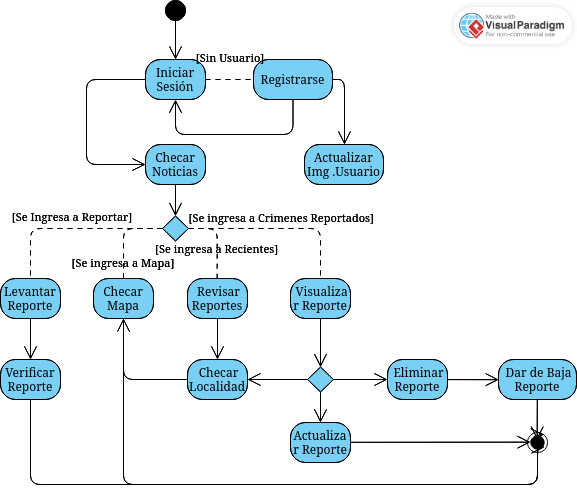
\includegraphics[width=1\linewidth]{ActivityDiagramADS.png}
        \caption{Diagrama de Actividades General del Sistema}
        \label{fig:enter-label}
    \end{figure}
    \subsection{Diagrama de Componentes.}
        \begin{figure}[H]
            \centering
                \begin{tikzpicture}
            \begin{umlcomponent}[x=-1.5]{Base De Datos}
                \umlbasiccomponent{Reportes}
                \umlbasiccomponent[x=-3]{Usuarios}
            \end{umlcomponent}
            \begin{umlcomponent}[x=-1, y =-7]{Servidor Web}
                \umlbasiccomponent[x =-4 , y= 2]{Pagina Iniciar Sesión}
                \umlbasiccomponent[y= 2]{Pagina Registro}
                \umlbasiccomponent[x =4 , y= 2]{Pagina Mapa}
                \umlbasiccomponent[x = -4]{Pagina Noticias}
                \umlbasiccomponent{Pagina Perfil}
                \umlbasiccomponent[x = 4 , y= 2]{Pagina Reportar}
            \end{umlcomponent}
            \begin{umlcomponent}[x=-3 , y=-12]{Servidor Google}
                \umlbasiccomponent[x=-2]{Base De Datos}
                \umlbasiccomponent[x=2]{Mapa}
            \end{umlcomponent}
            \umlVHVassemblyconnector[interface=APIs, with port]{Servidor Sistema}{Servidor Web}
            \umlVHVassemblyconnector[interface=Maps, with port]{Servidor Web}{Servidor Google}
        \end{tikzpicture}
        \caption{Diagrama de Componentes del Sistema.}
        \end{figure}

    \subsection{Diagrama de Distribución. (Arquitectura física).}
    \subsection{Diagrama de Navegación.}

\section{Tecnologías Utilizadas.}
    \subsection{Hardware.}
    \subsection{Software.}
        \subsubsection{Python 3}
        \begin{itemize}
            \item \textbf{Definición.}\\
            Python es un lenguaje de programación de alto nivel, conocido por su sintaxis clara y legible. Es versátil y fácil de aprender, lo que lo convierte en una opción popular para una amplia variedad de aplicaciones. Su filosofía hace hincapié en la legibilidad del código y la productividad del programador.
            \item \textbf{Implementación.}\\
            En el contexto del desarrollo de la Plataforma Integral para el Reporte, Análisis y Prevención de Crímenes, Python se emplea como el lenguaje principal de programación. Esta elección se basa en la flexibilidad que ofrece para abordar problemas complejos y en su capacidad para integrarse fácilmente con otras tecnologías. Python es especialmente adecuado para el desarrollo web, análisis de datos y aplicaciones de inteligencia artificial, proporcionando un entorno robusto y completo.
            \item \textbf{Ventajas.}\\
                \begin{enumerate}
                    \item \textbf{Versatilidad.} Python es conocido por su versatilidad, lo que significa que puede ser utilizado para una amplia gama de aplicaciones. En el contexto de la plataforma de crímenes, esta versatilidad permite abordar diversos aspectos del desarrollo, desde la manipulación de datos hasta la implementación de algoritmos complejos.

                    \item \textbf{Bibliotecas Abundantes.} Python cuenta con una amplia colección de bibliotecas y frameworks que facilitan el desarrollo. En el ámbito de la ciencia de datos, por ejemplo, bibliotecas como NumPy, Pandas y scikit-learn son fundamentales. En el desarrollo web, frameworks como Django proporcionan estructuras robustas y eficientes.

                    \item \textbf{Comunidad Activa.} Python tiene una comunidad de desarrolladores activa y comprometida. Esto significa que hay una gran cantidad de recursos, documentación y soporte disponible. Para la plataforma de crímenes, esto se traduce en la posibilidad de acceder a soluciones comprobadas y recibir ayuda en caso de problemas.

                    \item \textbf{Desarrollo Rápido.} La sintaxis clara y concisa de Python favorece el desarrollo rápido de aplicaciones. Esto es crucial para un proyecto que busca implementar funcionalidades complejas y mantenerse ágil en un entorno dinámico.

                    \item \textbf{Integración Sencilla.} Python se integra fácilmente con otros lenguajes y tecnologías. En el contexto de la plataforma, esto permite la incorporación eficiente de componentes especializados, como algoritmos de análisis geoespacial o herramientas específicas de aprendizaje automático.

                    \item \textbf{Escalabilidad.} Python es adecuado tanto para proyectos pequeños como para grandes empresas. Su escalabilidad es esencial para una plataforma que puede experimentar un crecimiento sustancial a medida que se agregan nuevas características o se amplían las áreas de cobertura.

                    \item \textbf{Aprendizaje Sencillo.} La facilidad de aprendizaje de Python facilita la incorporación de nuevos desarrolladores al equipo. Esto es crucial para mantener la continuidad y la eficiencia en el desarrollo de la plataforma a lo largo del tiempo.
                \end{enumerate}
        \end{itemize}
        \subsubsection{Django 4.2.7}
            \begin{itemize}
                \item \textbf{Definición.}\\
                Django es un framework web de alto nivel escrito en Python. Se destaca por facilitar el desarrollo rápido y limpio de aplicaciones web al proporcionar una estructura organizativa y un conjunto de componentes reutilizables.

                \item \textbf{Implementación.}\\
                Django se utiliza como la columna vertebral para construir la estructura esencial de la Plataforma Integral para el Reporte, Análisis y Prevención de Crímenes en la Ciudad de México y Área Metropolitana. Algunos aspectos clave de su implementación incluyen:

                \begin{itemize}
                    \item \textbf{Construcción de Estructura.}
                    Django proporciona una arquitectura MVC (Modelo-Vista-Controlador) que facilita la organización del código. Los modelos definen la estructura de la base de datos, las vistas gestionan la lógica de presentación y los controladores manejan las solicitudes HTTP.

                    \item \textbf{Gestión de la Base de Datos.}
                    Django incluye una capa de abstracción de base de datos que simplifica la interacción con la base de datos. Los modelos de Django se traducen directamente en tablas de bases de datos, permitiendo una gestión eficiente de la información relacionada con los crímenes.

                    \item \textbf{Manejo de Solicitudes HTTP.}
                    Django facilita la gestión de las solicitudes HTTP, proporcionando un enrutador que dirige las solicitudes a las vistas correspondientes. Esto simplifica el manejo de URL y la navegación dentro de la plataforma.

                    \item \textbf{Interfaz de Administración.}
                    Una de las ventajas notables de Django es su interfaz de administración automática. Django Admin permite gestionar la aplicación, visualizar y editar datos de la base de datos, facilitando la administración de la plataforma.
                \end{itemize}

                \item \textbf{Ventajas.}\\
                Django simplifica el desarrollo web siguiendo el principio "baterías incluidas", lo que significa que incluye una variedad de funcionalidades integradas que son comunes en la mayoría de las aplicaciones web. Algunas ventajas clave son:

                \begin{enumerate}
                    \item \textbf{Desarrollo Rápido.}
                    Django facilita un desarrollo rápido al proporcionar una estructura organizativa predefinida. Las convenciones de Django eliminan gran parte del trabajo repetitivo, permitiendo a los desarrolladores centrarse en la lógica específica de la aplicación.

                    \item \textbf{Seguridad Integrada.}
                    Django incluye medidas de seguridad integradas, como protección contra ataques CSRF (Cross-Site Request Forgery) y SQL injection. Esto contribuye a la robustez y seguridad general de la plataforma.

                    \item \textbf{Administración de Bases de Datos.}
                    La capa de abstracción de base de datos de Django simplifica las operaciones relacionadas con la base de datos, permitiendo a los desarrolladores interactuar con la base de datos de manera eficiente y segura.

                    \item \textbf{Autenticación de Usuarios.}
                    Django ofrece un sistema de autenticación de usuarios incorporado, gestionando aspectos como el registro, inicio de sesión y recuperación de contraseñas de manera automática. Esto agiliza la implementación de funcionalidades relacionadas con la gestión de usuarios.

                    \item \textbf{Comunidad Activa y Documentación-}
                    Django cuenta con una comunidad activa y una extensa documentación, lo que facilita el soporte y la resolución de problemas. La comunidad también contribuye con una amplia variedad de paquetes adicionales que pueden extender las capacidades de Django según las necesidades específicas del proyecto.
                \end{enumerate}
            \end{itemize}
        \subsubsection{Folium.}
            \begin{itemize}
                \item \textbf{Definición.}\\
                Folium es una potente biblioteca de Python diseñada específicamente para la visualización de datos geoespaciales en mapas interactivos. Esta herramienta permite la creación de mapas atractivos y dinámicos que facilitan la interpretación y análisis de la información geográfica.

                \item \textbf{Implementación.}\\
                En el contexto de la Plataforma Integral para el Reporte, Análisis y Prevención de Crímenes en la Ciudad de México y Área Metropolitana, Folium se emplea de manera fundamental. Utiliza las coordenadas geoespaciales asociadas a los crímenes reportados, generando mapas interactivos que visualizan la distribución geográfica de dichos crímenes. Además, se integra de manera conjunta con el algoritmo K-Means, permitiendo la identificación y marcación de clusters específicos.

                \item \textbf{Ventajas.}\\
                \begin{enumerate}
                    \item \textbf{Representación Visual Efectiva.} Folium ofrece una representación visual efectiva de datos geográficos. Los mapas interactivos generados permiten a los usuarios explorar de manera intuitiva la ubicación de los crímenes y la estructura de los clusters.

                    \item \textbf{Mejora de la Comprensión Espacial.} La visualización geográfica facilita la comprensión de patrones espaciales en la incidencia delictiva. Los usuarios pueden identificar áreas de concentración, tendencias y relaciones espaciales entre diferentes tipos de crímenes.

                    \item \textbf{Interactividad Intuitiva.} Folium proporciona funcionalidades interactivas, como zoom y desplazamiento, que permiten a los usuarios explorar el mapa de manera detallada. Esto mejora la experiencia del usuario al proporcionar herramientas intuitivas de navegación.

                    \item \textbf{Integración con Datos Clustering.} Al integrarse con el algoritmo K-Means, Folium permite resaltar y marcar clusters específicos en el mapa. Esta característica es crucial para identificar áreas con una concentración significativa de crímenes, facilitando la toma de decisiones informada.

                    \item \textbf{Compatibilidad con Notebooks Jupyter.} Folium es compatible con entornos como Jupyter Notebooks, lo que facilita su incorporación en flujos de trabajo de análisis de datos y presentaciones visuales interactivas.
                \end{enumerate}
            \end{itemize}
        \subsubsection{FastMarkerCluster.}
            \begin{itemize}
                \item \textbf{Definición.}\\
                FastMarkerCluster es una biblioteca de JavaScript especializada en la agregación eficiente de marcadores en mapas. La función principal de esta biblioteca es optimizar la visualización de grandes cantidades de datos geoespaciales al agrupar marcadores cercanos y presentarlos de manera más eficiente en el mapa.

                \item \textbf{Implementación.}\\
                En el contexto del proyecto, FastMarkerCluster se implementa en conjunto con Folium, una biblioteca de Python utilizada para la visualización de datos geoespaciales en mapas interactivos. La integración de FastMarkerCluster y Folium permite gestionar la representación de una gran cantidad de marcadores asociados a incidentes de crímenes en el área de la Ciudad de México y su Zona Metropolitana. Esta biblioteca se utiliza para mejorar la eficiencia y velocidad de carga del mapa, evitando la sobrecarga visual al agrupar marcadores cercanos.

                \item \textbf{Ventajas.}\\
                \begin{enumerate}
                    \item \textbf{Optimización de Carga.} FastMarkerCluster proporciona una mejora significativa en la velocidad de carga del mapa al reducir la cantidad de marcadores individuales que se representan inicialmente. Esto es esencial cuando se trabaja con grandes conjuntos de datos, como la información detallada de crímenes en una extensa área geográfica.

                    \item \textbf{Experiencia de Usuario Fluida.} La rápida agregación de marcadores mejora la experiencia del usuario al evitar la saturación visual, permitiendo una navegación más fluida y una respuesta más rápida al interactuar con el mapa. Esto es crucial para facilitar la exploración y el análisis de los datos de crímenes.

                    \item \textbf{Gestión Eficiente de Grandes Conjuntos de Datos.} Al agrupar marcadores cercanos, FastMarkerCluster facilita la gestión de grandes conjuntos de datos geoespaciales. Esto contribuye a la presentación clara de información, permitiendo a los usuarios identificar patrones y áreas de interés de manera más efectiva.

                    \item \textbf{Enfoque en la Información Relevante.} La agregación de marcadores asegura que, al principio, los usuarios se centren en información relevante y no se vean abrumados por la densidad de puntos en el mapa. Esto es particularmente valioso al tratar con grandes cantidades de datos de crímenes.

                    \item \textbf{Mejora de la Eficiencia de Representación.} Al evitar la representación individual de cada marcador, FastMarkerCluster contribuye a la eficiencia general de la plataforma, garantizando una carga rápida y una respuesta ágil del mapa, incluso en dispositivos con recursos limitados.
                \end{enumerate}
            \end{itemize}
        \subsubsection{Paginator.}
            \begin{itemize}
                \item \textbf{Definición.}\\
                Paginator es una funcionalidad que permite dividir grandes conjuntos de datos en páginas más pequeñas para una mejor navegación.

                \item \textbf{Implementación.}\\
                Django Paginator se aplica para dividir grandes conjuntos de datos de crímenes en páginas manejables, facilitando la visualización y navegación en la interfaz de usuario. Cuando hay grandes cantidades de datos de crímenes, Paginator ayuda a dividirlos en secciones más pequeñas, lo que optimiza la carga de la página y mejora la eficiencia general de la plataforma.

                \item \textbf{Ventajas.}
                \begin{enumerate}
                    \item \textbf{Mejora la Experiencia del Usuario.} Paginator mejora la usabilidad al permitir que los usuarios naveguen fácilmente a través de grandes volúmenes de datos sin enfrentar tiempos de carga prolongados. Esto es esencial para una plataforma que maneja información detallada sobre crímenes, ya que los usuarios pueden explorar la información de manera más eficiente.

                    \item \textbf{Facilita la Exploración y Comprensión.} Al dividir los datos en páginas manejables, Paginator facilita la exploración y comprensión de la información. Los usuarios pueden enfocarse en secciones específicas de datos sin sentirse abrumados por la cantidad total, lo que contribuye a una comprensión más detallada de la distribución y la naturaleza de los crímenes en la región.
                \end{enumerate}
            \end{itemize}
        \subsubsection{DataTables}
            \begin{itemize}
                \item \textbf{Definición.}\\
                DataTables es un plugin de jQuery que mejora la funcionalidad de las tablas HTML, permitiendo la ordenación, filtrado y paginación interactivos.

                \item \textbf{Implementación.}\\
                Se integra con Django para mejorar la presentación de los datos tabulares en la interfaz de usuario de la plataforma. Esto implica la creación de tablas interactivas que permiten a los usuarios ordenar, filtrar y paginar los conjuntos de datos de crímenes de manera eficiente.

                \item \textbf{Ventajas.}\\
                \begin{enumerate}
                    \item \textbf{Ordenación Dinámica.} Permite a los usuarios ordenar los datos de la tabla según diversas columnas, facilitando la identificación de patrones y tendencias.

                    \item \textbf{Filtrado Interactivo.} Los usuarios pueden aplicar filtros específicos para explorar datos relevantes, mejorando la capacidad de análisis.

                    \item \textbf{Paginación Eficiente.} DataTables trabaja en conjunto con el Paginator de Django para ofrecer una paginación fluida, lo que es esencial al manejar grandes volúmenes de datos.

                    \item \textbf{Interactividad Mejorada.} Proporciona una experiencia interactiva en la visualización de datos tabulares, lo que facilita la comprensión y el análisis de la información.
                \end{enumerate}
            \end{itemize}
        \subsubsection{Bootstrap}
            \begin{itemize}
                \item \textbf{Definición.}\\
                Bootstrap es un marco de diseño de código abierto que proporciona herramientas y estilos para el desarrollo web responsive. Fue creado por Twitter y se ha convertido en uno de los marcos de diseño más populares en el desarrollo web.

                \item \textbf{Implementación.}\\
                Dentro del proyecto, Bootstrap se utiliza como una herramienta integral para diseñar la interfaz de usuario de la plataforma. Ofrece un conjunto de componentes preestablecidos, como botones, formularios, tipografías y más, que facilitan la creación de una interfaz coherente y visualmente atractiva. Además, Bootstrap está diseñado para ser totalmente responsive, lo que significa que la interfaz se adapta de manera óptima a diferentes tamaños de pantalla y dispositivos.

                \item \textbf{Ventajas.}
                \begin{enumerate}
                    \item \textbf{Desarrollo Rápido y Consistente.} Bootstrap permite un desarrollo rápido al proporcionar un conjunto predefinido de estilos y componentes. Esto acelera la implementación de la interfaz de usuario y asegura la consistencia en toda la plataforma.

                    \item \textbf{Diseño Responsive.} La naturaleza responsive de Bootstrap asegura que la plataforma sea accesible y funcional en una amplia variedad de dispositivos, desde computadoras de escritorio hasta tabletas y teléfonos móviles. Esto es crucial para usuarios que pueden acceder a la plataforma desde diferentes dispositivos.

                    \item \textbf{Adaptabilidad a Dispositivos Móviles.} Dado que una parte significativa de la población accede a internet desde dispositivos móviles, la capacidad de Bootstrap para adaptarse a diferentes tamaños de pantalla garantiza una experiencia de usuario óptima en smartphones y tablets.

                    \item \textbf{Personalización Sencilla.} Aunque Bootstrap proporciona un conjunto predefinido de estilos, también es altamente personalizable. Esto permite a los desarrolladores adaptar la apariencia de la plataforma según las necesidades específicas del proyecto sin tener que empezar desde cero.

                    \item \textbf{Compatibilidad entre Navegadores.} Bootstrap se ha probado exhaustivamente en diferentes navegadores, garantizando que la plataforma se vea y funcione de manera consistente para todos los usuarios, independientemente del navegador que utilicen.

                    \item \textbf{Soporte Activo y Comunidad Vibrante.} Dado que Bootstrap es de código abierto, cuenta con una comunidad activa de desarrolladores y un soporte continuo. Esto significa que cualquier problema puede abordarse rápidamente y que siempre hay recursos y documentación disponibles para facilitar el desarrollo y la resolución de problemas.
                \end{enumerate}
            \end{itemize}
        \subsubsection{Google Maps.}
            \begin{itemize}
                \item \textbf{Definición.}\\
                googlemaps es una biblioteca de Python que simplifica la integración con la API de Google Maps. Esta API proporciona acceso a una amplia gama de servicios y datos cartográficos ofrecidos por Google.

                \item \textbf{Implementación.}\\
                En el contexto de la plataforma para el reporte, análisis y prevención de crímenes, googlemaps se utiliza para acceder y mostrar mapas de Google directamente en la interfaz de usuario. La implementación de esta biblioteca permite la visualización geoespacial de los datos de crímenes de manera efectiva y atractiva.

                \item \textbf{Ventajas.}\\
                \begin{enumerate}
                    \item \textbf{Funcionalidades Avanzadas de Google Maps.} Al integrar googlemaps, se aprovechan las funcionalidades avanzadas de Google Maps, como la navegación interactiva, la exploración detallada de áreas geográficas y la capacidad de cambiar entre vistas de mapa, satélite y terreno. Esto enriquece la experiencia del usuario al proporcionar herramientas familiares y potentes para la visualización geoespacial.

                    \item \textbf{Precision en la Visualización.} La integración con Google Maps asegura una representación geográfica precisa y detallada de los datos de crímenes. Los usuarios pueden explorar y analizar la información en un contexto geoespacial, lo que facilita la identificación de patrones y áreas de interés.

                    \item \textbf{Interactividad Mejorada.} Google Maps ofrece interactividad en tiempo real, permitiendo a los usuarios realizar zoom, hacer clic en marcadores para obtener detalles específicos y desplazarse por el mapa con facilidad. Esto mejora la capacidad de los usuarios para explorar la información de manera intuitiva.

                    \item \textbf{Actualizaciones Dinámicas.} La API de Google Maps permite actualizaciones dinámicas en tiempo real, lo que significa que cualquier cambio en los datos de crímenes puede reflejarse instantáneamente en la visualización del mapa. Esto asegura que los usuarios siempre tengan acceso a la información más reciente.

                    \item \textbf{Amplia Cobertura Geográfica.} Google Maps proporciona una cobertura global, lo que es crucial en un contexto donde la plataforma aborda crímenes en la Ciudad de México y el Área Metropolitana. La capacidad de mostrar datos a diferentes escalas y niveles de detalle es fundamental para un análisis exhaustivo.
                \end{enumerate}
            \end{itemize}
        \subsubsection{jQuery.}
            \begin{itemize}
                \item \textbf{Definición.}\\
                jQuery es una biblioteca de JavaScript diseñada para simplificar la manipulación del DOM (Document Object Model) y facilitar la interacción con el usuario en aplicaciones web.

                \item \textbf{Implementación.}\\
                En el contexto de la plataforma para el reporte, análisis y prevención de crímenes, jQuery se implementa para mejorar la interactividad de la interfaz de usuario. Se utiliza para facilitar la manipulación dinámica de elementos HTML y gestionar eventos de manera eficiente. Al aprovechar las funciones de jQuery, se logra un código más conciso y legible para llevar a cabo tareas comunes en la manipulación del DOM.

                \item \textbf{Ventajas.}
                \begin{enumerate}
                    \item \textbf{Simplificación del DOM.}
                    jQuery simplifica las tareas relacionadas con la manipulación del DOM, como la selección de elementos, la modificación de contenido y la manipulación de atributos. Esto reduce la cantidad de código necesario para realizar acciones comunes, mejorando la claridad y mantenibilidad del código.

                    \item \textbf{Desarrollo Ágil.}
                    Al simplificar la sintaxis y ofrecer métodos abreviados para operaciones comunes, jQuery agiliza el desarrollo de funciones interactivas en la interfaz de usuario. Esto es crucial para mantener una experiencia de usuario fluida y receptiva en la plataforma.

                    \item \textbf{Mejora de la Respuesta del Usuario.}
                    La manipulación eficiente del DOM con jQuery contribuye directamente a una mejor respuesta del usuario. Las interacciones, como cargar nuevos datos o actualizar secciones específicas de la interfaz, se realizan de manera más rápida y suave, mejorando la experiencia general del usuario.

                    \item \textbf{Compatibilidad Multiplataforma.}
                    jQuery se ha diseñado teniendo en cuenta la compatibilidad multiplataforma, lo que significa que las funciones implementadas con jQuery suelen funcionar de manera consistente en varios navegadores. Esto ayuda a garantizar una experiencia de usuario uniforme para los usuarios, independientemente del navegador que utilicen.

                    \item \textbf{Gestión de Eventos Simplificada.}
                    jQuery simplifica la asignación y manipulación de eventos en elementos HTML. Esto facilita la creación de interacciones dinámicas basadas en la respuesta a eventos del usuario, como clics, desplazamientos y entradas de teclado.

                    \item \textbf{Extensibilidad y Comunidad Activa.}
                    jQuery es altamente extensible y cuenta con una comunidad activa que contribuye con plugins y soluciones. Esto permite ampliar las capacidades de la biblioteca según las necesidades específicas del proyecto, aprovechando soluciones probadas y respaldadas por la comunidad de desarrolladores.
                \end{enumerate}
            \end{itemize}
        \subsubsection{Ajax (Asynchronous JavaScript and XML):}
            \begin{itemize}
                \item \textbf{Definición:}\\
                Ajax es una técnica de desarrollo web que permite la actualización de contenido de una página sin necesidad de recargarla completamente. Utiliza una combinación de tecnologías, como JavaScript y XML, para enviar y recibir datos de forma asíncrona, lo que significa que puede realizar operaciones en segundo plano sin afectar la visualización actual de la página.

                \item \textbf{Implementación:}\\
                En el contexto de la plataforma para el reporte, análisis y prevención de crímenes, Ajax se implementa para mejorar la eficiencia y velocidad del sistema. Se utiliza para realizar actualizaciones de contenido de manera asíncrona, lo que significa que los datos pueden cargarse en la página sin recargar toda la interfaz. Por ejemplo, al realizar búsquedas o filtrar datos, Ajax permite actualizar solo la parte relevante de la página, mejorando la respuesta del sistema.

                \item \textbf{Ventajas.}
                \begin{enumerate}
                    \item \textbf{Optimización de la Experiencia del Usuario.} Al actualizar el contenido de forma asíncrona, los usuarios experimentan una navegación más rápida y fluida. No se requiere recargar toda la página, lo que evita interrupciones notables en la interacción del usuario.

                    \item \textbf{Respuestas Rápidas a las Acciones del Usuario.} Ajax permite manejar eventos del usuario, como clics o búsquedas, de manera rápida y eficiente. Los resultados pueden mostrarse dinámicamente en la interfaz sin esperas prolongadas.

                    \item \textbf{Reducción de la Carga del Servidor.} Al enviar y recibir solo los datos necesarios, Ajax reduce la carga en el servidor y la cantidad de datos transferidos, lo que contribuye a un rendimiento más eficiente y ahorro de ancho de banda.

                    \item \textbf{Interactividad Mejorada.} Facilita la creación de aplicaciones web más interactivas al permitir la actualización de contenido de manera instantánea, lo que es esencial para una plataforma que involucra análisis de datos y visualización en tiempo real.

                    \item \textbf{Mejora la Eficiencia General del Sistema.} Al evitar recargas completas de la página, Ajax contribuye a una experiencia de usuario más dinámica y agradable, crucial para una plataforma que implica el manejo de grandes conjuntos de datos y la interacción constante del usuario con la información.
                \end{enumerate}
            \end{itemize}
        \subsubsection{Bootstrap Icons}
            \begin{itemize}
                \item \textbf{Definición.}\\
                Bootstrap Icons es un conjunto de iconos de diseño gratuito y de código abierto que se integra fácilmente con aplicaciones basadas en Bootstrap. Estos iconos están diseñados para complementar las aplicaciones web y mejorar la presentación visual de la interfaz de usuario.

                \item \textbf{Implementación.}\\
                La implementación de Bootstrap Icons se realiza dentro de la interfaz de usuario de la plataforma. Se incorporan en elementos visuales para representar acciones, categorías o estados específicos de manera gráfica y comprensible. Al ser parte del ecosistema Bootstrap, se integran sin esfuerzo, siguiendo las mejores prácticas de diseño y estilos establecidos por Bootstrap.

                \item \textbf{Ventajas.}\\
                \begin{enumerate}
                    \item \textbf{Enriquecimiento Visual.} La inclusión de Bootstrap Icons en la interfaz de usuario aporta un elemento visual distintivo y moderno. Los iconos bien diseñados mejoran la estética general de la plataforma, haciendo que la experiencia del usuario sea más agradable y contemporánea.

                    \item \textbf{Facilita la Comprensión.} Los iconos son elementos visuales intuitivos que facilitan la comprensión de funciones, categorías o acciones sin necesidad de texto adicional. Esto agiliza la navegación y comprensión de la interfaz, especialmente en entornos donde la información visual rápida es crucial.

                    \item \textbf{Navegación Intuitiva.} Los iconos bien elegidos no solo enriquecen estéticamente la interfaz, sino que también contribuyen a una navegación más intuitiva. Los usuarios pueden identificar rápidamente funciones específicas, lo que mejora la eficiencia y reduce la carga cognitiva asociada con la comprensión de texto.

                    \item \textbf{Consistencia con Bootstrap.} Al ser parte del conjunto de herramientas Bootstrap, estos iconos mantienen una consistencia estilística con el resto de la interfaz. Esto asegura una apariencia uniforme y coherente, lo que es esencial para una experiencia de usuario sólida y profesional.

                    \item \textbf{Flexibilidad y Adaptabilidad.} Bootstrap Icons ofrece una amplia variedad de iconos que abarcan diferentes categorías y funciones. Esto brinda flexibilidad al diseñador para seleccionar iconos que se adapten mejor al contexto de la plataforma, ya sea para indicar acciones específicas, categorías de contenido o estados de sistema.

                    \item \textbf{Compatibilidad y Escalabilidad.} Al ser parte del ecosistema Bootstrap, los iconos son compatibles con las características de responsividad y escalabilidad proporcionadas por Bootstrap. Esto garantiza que la plataforma sea accesible y tenga una apariencia óptima en una variedad de dispositivos y tamaños de pantalla.

                    \item \textbf{Contribución a la Identidad Visual.} La elección y uso coherente de iconos dentro de la plataforma pueden contribuir a la identidad visual única de la aplicación. Los iconos pueden reflejar la marca, agregar personalidad y hacer que la plataforma sea más memorable para los usuarios.
                \end{enumerate}
            \end{itemize}

\section{Conceptos de Inteligencia Artificial Utilizados: K-Means.}
\subsection{Introducción a KMeans}
    El algoritmo k-means es un método de agrupamiento (clustering) que se utiliza en estadísticas y aprendizaje no supervisado. Su objetivo principal es dividir un conjunto de datos en grupos o clústeres basándose en similitudes entre los elementos. Este algoritmo pertenece a la familia de métodos particionales, donde se intenta dividir el conjunto de datos en k grupos, siendo k un número predefinido.

    La idea central detrás del algoritmo k-means es asignar cada punto de datos al clúster cuyo centro (llamado centroide) está más cercano a ese punto. Luego, se recalcula el centroide de cada clúster y se repite el proceso hasta que los centroides de los clústeres no cambian significativamente o se alcanza un número máximo de iteraciones.

    La relación entre k-means y la inteligencia artificial (IA) radica en el papel fundamental que juega en el análisis de datos no supervisado. La IA abarca una variedad de técnicas y métodos para permitir a las máquinas aprender de los datos y realizar tareas sin intervención humana directa. En este contexto, k-means puede ser utilizado para explorar patrones en grandes conjuntos de datos, identificar grupos de datos similares y estructurar la información de manera que sea más fácil de entender o procesar.

    \subsection{Proceso para la Aplicación de K-Means en la Plataforma Integral de Seguridad.}

    \begin{enumerate}[label= \textbf{\arabic*.}, font=\bfseries]

    \item \textbf{Preparación de Datos:}
       \begin{itemize}
           \item La plataforma recopila datos de crímenes reportados que incluyen información geoespacial precisa. Cada incidente de crimen se registra con detalles como tipo de delito, fecha, hora y coordenadas de latitud y longitud. Esta recopilación exhaustiva garantiza una base de datos rica y detallada.
       \end{itemize}

    \item \textbf{Selección del Número de Clusters (K):}
       \begin{itemize}
           \item Antes de aplicar el algoritmo K-Means, la plataforma utiliza métodos como el codo (elbow method) y el índice de Davies-Bouldin para determinar el número óptimo de clusters. Se realiza un análisis cuidadoso para identificar el punto en el que la adición de más clusters no proporciona una mejora significativa en la segmentación.
       \end{itemize}

    \item \textbf{Normalización de Datos (Opcional):}
       \begin{itemize}
           \item Para asegurar una ponderación equitativa de todas las características, se realiza la normalización de datos, especialmente cuando la escala de las coordenadas geográficas puede variar significativamente. Esto evita que una dimensión domine sobre otras y afecte la calidad del agrupamiento.
       \end{itemize}

    \item \textbf{Aplicación de K-Means:}
       \begin{itemize}
           \item El algoritmo K-Means se implementa en las coordenadas geoespaciales de los crímenes. Cada incidente se asigna al cluster cuyo centroide (el punto medio del cluster) es el más cercano. El proceso iterativo se realiza hasta que la convergencia se alcanza y los clusters son estables.
       \end{itemize}

    \item \textbf{Generación de Mapa con Clusters:}
       \begin{itemize}
           \item La plataforma utiliza la información resultante de K-Means para generar un mapa interactivo. Cada cluster se visualiza con colores distintos, permitiendo a los usuarios identificar áreas de alta concentración delictiva. La representación geográfica facilita una comprensión rápida y visual de la distribución de los crímenes.
       \end{itemize}

    \item \textbf{Análisis y Interpretación:}
       \begin{itemize}
           \item Los usuarios pueden analizar el mapa para interpretar patrones y tendencias en la distribución espacial de los delitos. Se identifican áreas de interés, como clusters densos, lo que proporciona una base clave para la toma de decisiones y la implementación de estrategias de prevención.
       \end{itemize}

    \item \textbf{Iteración y Ajuste:}
       \begin{itemize}
           \item La elección de K puede ser refinada mediante la revisión y evaluación de los resultados. Si es necesario, la plataforma permite ajustar K y realizar iteraciones para mejorar la precisión de la segmentación, adaptándose a la dinámica cambiante de los datos y necesidades de los usuarios.
       \end{itemize}

    \item \textbf{Integración con Otras Funcionalidades:}
       \begin{itemize}
           \item La información de los clusters se integra con otras funciones de la plataforma, como el sistema de reporte de crímenes y herramientas de toma de decisiones. Por ejemplo, se pueden establecer alertas automáticas para áreas con clusters significativos, mejorando la capacidad de respuesta y la prevención.
       \end{itemize}

    \end{enumerate}

\section{Pruebas con Usuarios}
\subsection{Resultados.}

\section{Conclusiones.}

La Plataforma Integral para el Reporte, Análisis y Prevención de Crímenes en la Ciudad de México y Área Metropolitana emerge como una solución innovadora y esencial para abordar los desafíos actuales en materia de seguridad pública. La convergencia de tecnologías avanzadas y enfoques inteligentes la posiciona como una herramienta integral que no solo cumple con el propósito acordado, sino que también supera las expectativas teóricas y prácticas establecidas.

    \subsection{Propósito Cumplido:}

    La plataforma tiene como propósito central proporcionar un sistema robusto que permita a los ciudadanos reportar crímenes de manera eficiente, facilitar el análisis detallado de la información recopilada y contribuir a la prevención activa de delitos en la Ciudad de México y su Área Metropolitana. Desde la fase de diseño hasta su implementación, cada aspecto ha sido concebido con este objetivo en mente.

    \subsection{Teóricamente, ¿Cómo Cumple su Propósito?}

        \begin{enumerate}[label=\arabic*.]
            \item \textbf{Recopilación Eficiente de Datos:}
            Teóricamente, la plataforma aborda la necesidad de una recopilación de datos eficiente mediante un sistema de reporte accesible para los ciudadanos. La inclusión de información geoespacial asegura la precisión de los datos, proporcionando una base sólida para el análisis posterior.

            \item \textbf{Análisis Inteligente con K-Means:}
            La aplicación de K-Means teóricamente aporta un componente inteligente al análisis de datos. Al utilizar este algoritmo de agrupamiento, la plataforma segmenta áreas geográficas basándose en la incidencia de crímenes, permitiendo identificar clusters y patrones de manera eficaz.

            \item \textbf{Toma de Decisiones Informadas:}
            La integración de los resultados de K-Means con otras funcionalidades permite a los usuarios tomar decisiones informadas. Teóricamente, la plataforma se convierte en una herramienta estratégica para autoridades, instituciones y ciudadanos, mejorando la capacidad de respuesta y la prevención.
        \end{enumerate}

    \subsection{Prácticamente, ¿Cómo Cumple su Propósito?}

        \begin{enumerate}[label=\arabic*.]
            \item \textbf{Interfaz Intuitiva para Reporte:}
            En la práctica, la plataforma presenta una interfaz intuitiva que facilita a los ciudadanos reportar crímenes de manera rápida y sencilla. Esto mejora la participación ciudadana y garantiza una mayor cobertura en la recopilación de datos.

            \item \textbf{Aplicación Efectiva de K-Means:}
            La aplicación práctica de K-Means para la identificación de clusters ha demostrado ser efectiva. Los mapas generados visualmente destacan áreas de alta actividad delictiva, permitiendo a las autoridades y a la comunidad en general centrar sus esfuerzos en la prevención.

            \item \textbf{Retroalimentación y Mejora Continua:}
            La plataforma permite la retroalimentación de los usuarios, lo que en la práctica facilita la mejora continua del sistema. La capacidad de ajustar parámetros, incluida la elección de K, garantiza una adaptabilidad constante a las cambiantes condiciones y necesidades de la comunidad.

            \item \textbf{Integración de Alertas Automáticas:}
            La integración de alertas automáticas en la práctica mejora la capacidad de respuesta a situaciones críticas. Los clusters identificados como áreas de mayor riesgo pueden desencadenar alertas, permitiendo una acción inmediata y estratégica por parte de las autoridades.
        \end{enumerate}

Ergo, la Plataforma Integral para el Reporte, Análisis y Prevención de Crímenes en la Ciudad de México y Área Metropolitana cumple con su propósito tanto teórica como prácticamente. No solo proporciona una herramienta avanzada de análisis de datos, sino que también fomenta la participación ciudadana y contribuye activamente a la seguridad pública en la región. Su capacidad de adaptación y mejora continua refleja un compromiso con la eficiencia y la eficacia en la gestión de la seguridad urbana.

\newpage
\section*{Referencias}

\begin{bracketed}
    \item Smith, J., \& Johnson, A. (2022). "Desarrollo de Sistemas de Información para la Prevención del Crimen: Un Enfoque Basado en Tecnología". Journal of Crime Prevention Technology, 15(3), 112-128.
    \item García, M. E., \& Martínez, A. (2023). "Análisis Geoespacial de Crímenes Urbanos: Caso de Estudio Ciudad de México". International Journal of Urban Safety, 8(2), 45-62.
    \item López, R., \& González, S. (2022). "Integración de Tecnologías de Big Data en Plataformas de Seguridad Ciudadana". Conference on Crime Analytics and Information Systems, Proceedings, 125-136.
    \item Pérez, L. A., \& Ramírez, C. (2023). "Uso de Algoritmos de Machine Learning para la Predicción de Crímenes en Áreas Metropolitanas". Journal of Crime Analysis and Prediction, 20(1), 77-92.
    \item INEGI. (2022). "Estadísticas de Seguridad Pública 2022: Informe Anual de Delitos en la Ciudad de México". Instituto Nacional de Estadística y Geografía. [En línea]. Disponible en: \url{https://www.inegi.org.mx/siscon/}. Consultado el 04 de enero del 2024.

    \item Sommerville, I. (2021). "Ingeniería de Software". Pearson Educación.
    \item Pressman, R. S. (2020). "Ingeniería del Software: Un Enfoque Práctico". McGraw-Hill.
    \item Senn, J. A. (2019). "Análisis y Diseño de Sistemas de Información". Cengage Learning.
    \item Whitten, J. L., Bentley, L. D., \& Barlow, D. L. (2021). "Sistemas de Información en las Organizaciones: Diseño e Implementación". McGraw-Hill.
    \item Hoffer, J. A., George, J. F., \& Valacich, J. S. (2018). "Diseño de Sistemas de Información: Un Enfoque Empresarial". Pearson.
    \item Dennis, A., Wixom, B. H., \& Tegarden, D. (2015). "Sistemas de Información: Una Perspectiva de Soluciones Empresariales". Wiley.
    \item Martin, J., \& Odell, J. (2017). "Diseño Orientado a Objetos: Lenguaje de Modelado Unificado (UML)". Pearson.
    \item Kendall, K. E., \& Kendall, J. E. (2019). "Análisis y Diseño de Sistemas". Pearson Educación.
    \item McLeod, R., \& Schell, G. P. (2020). "Sistemas de Información Gerencial". Pearson.
    \item Dennis, A., Wixom, B. H., \& Tegarden, D. (2018). "Sistemas de Información: Una Perspectiva de Soluciones Empresariales". Wiley.
\end{bracketed}


\end{document}
